\documentclass[11pt]{article}
\usepackage[top=2.2cm, bottom=3.cm, left=2.5cm, right=2.5cm]{geometry}
\usepackage[utf8]{inputenc}
\usepackage{amsmath,amsthm,amsfonts,amssymb,amscd}
\usepackage{lastpage}
\usepackage{graphicx}
\usepackage{natbib}
\usepackage{hyperref}
\nonstopmode

\bibliographystyle{aasjournal}

\setlength{\parindent}{0.0in}
\setlength{\parskip}{0.8em}
\renewcommand{\baselinestretch}{1.}

\hypersetup{%
  colorlinks=true,
  linkcolor=blue,
  linkbordercolor={0 0 1},
  citecolor=blue,
  urlcolor=black,
}

\newcommand{\code}{\texttt}

\begin{document}

\title{\textbf{Charting the Growth of Galaxies} \\[0.25cm] \large{CTA200H | 2020 Summer}}
\author{Jeff Shen \\ Advisor: Dr. Allison Man}
\date{\today}
\maketitle

\section*{Spectral Fitting}

Fig. \ref{fig:initial_spectra} shows the spectra for each of the three multiple images of Gal. 2 (Gal. 2a, 2b, and 2c) of the MS 0451.6−0305 cluster, as defined in \cite{MacKenzie2014}. The spectrum for Gal. 2a is noisy, and there is no distinct peak like the ones seen in the plots of the other two spectra. In the second and third panels of the figure, there are peaks in the intensity at a frequency of around 88 GHz. 

\begin{figure}[!htbp]
    \centering
    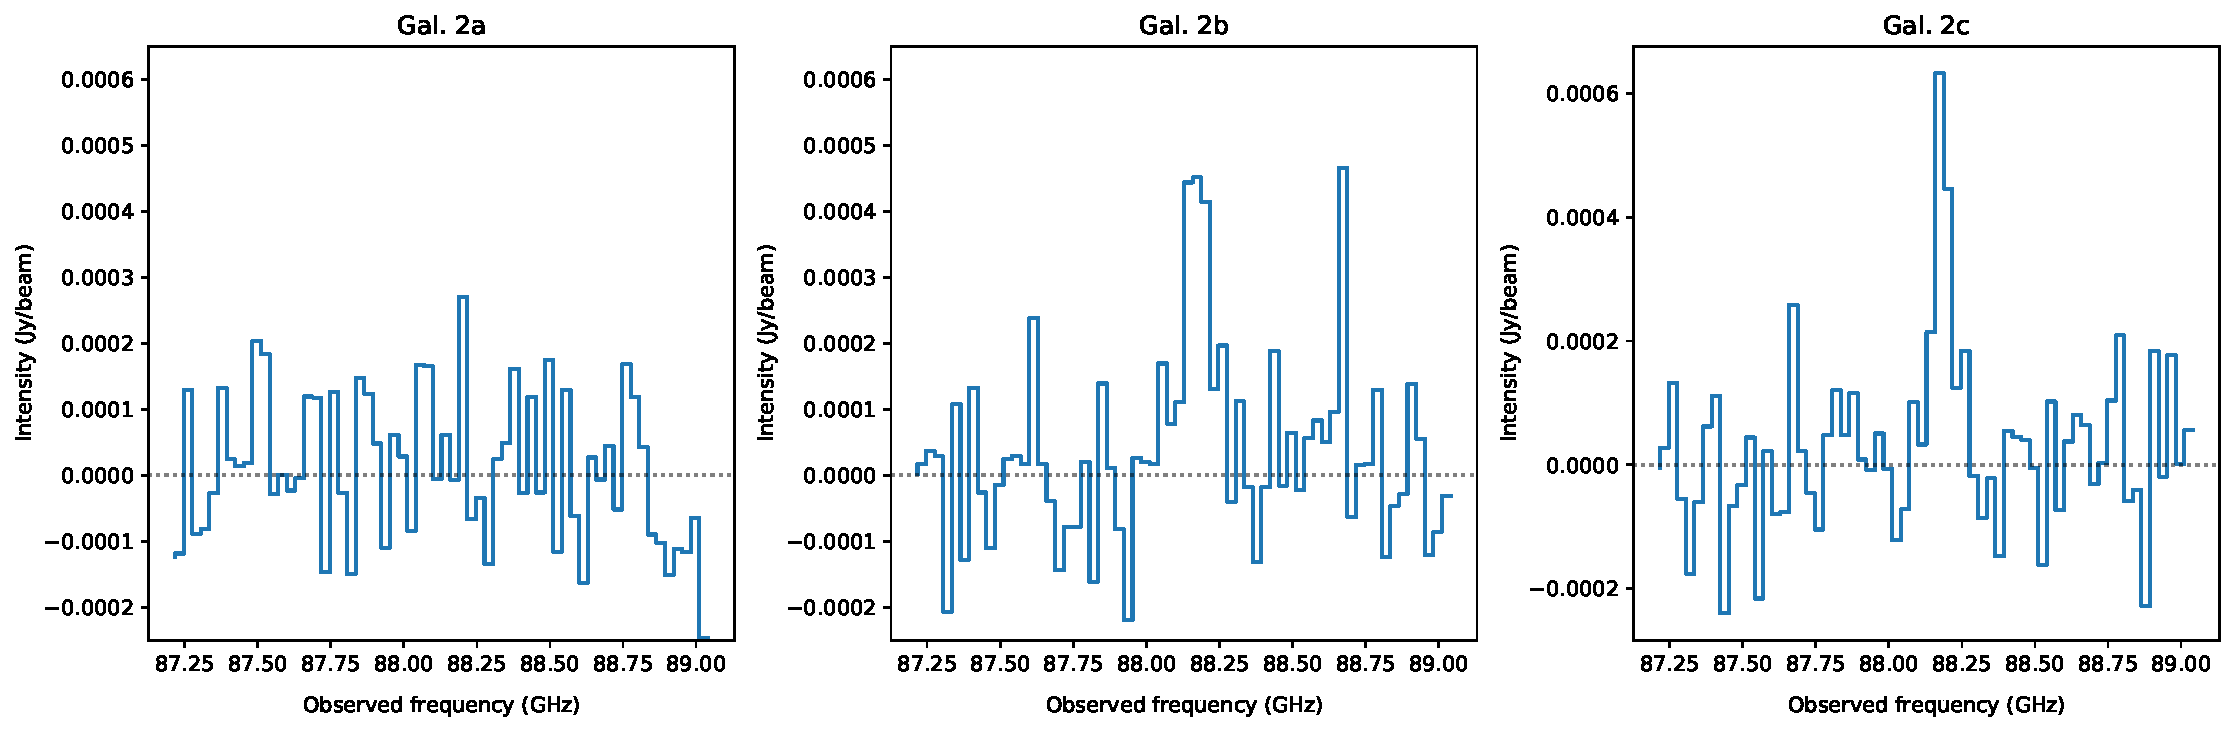
\includegraphics[width=\linewidth]{../figs/initial_spectra.pdf}
	\caption{Plot of the extracted spectra of the multiple images of Gal. 2. Observed frequency (GHz) is plotted against the intensity (Jy/beam).}
    \label{fig:initial_spectra}
\end{figure}

The Levenberg–Marquardt algorithm\footnote{\url{https://en.wikipedia.org/wiki/Levenberg-Marquardt_algorithm}} from \code{astropy.modeling}, which minimizes the sum of squared residuals (SSR), was used to fit a 1D Gaussian model to each of the spectra. The results are shown in Fig. \ref{fig:gaussian_fit}. As expected, the algorithm had some trouble identifying a distinct peak for Gal. 2a, and as a result, the fitted Gaussian line for that image is much broader and has a smaller amplitude than the lines for the other two images. Each fit yielded a standard deviation, and for a Gaussian, the FWHM can be calculated\footnote{\url{https://en.wikipedia.org/wiki/Full_width_at_half_maximum}} from the standard deviation $\sigma$ as 
\begin{align}\label{eqn:fwhm}
	\rm{FWHM} = 2\sqrt{2\log{2}}\sigma.
\end{align}

\begin{figure}[!htbp]
    \centering
	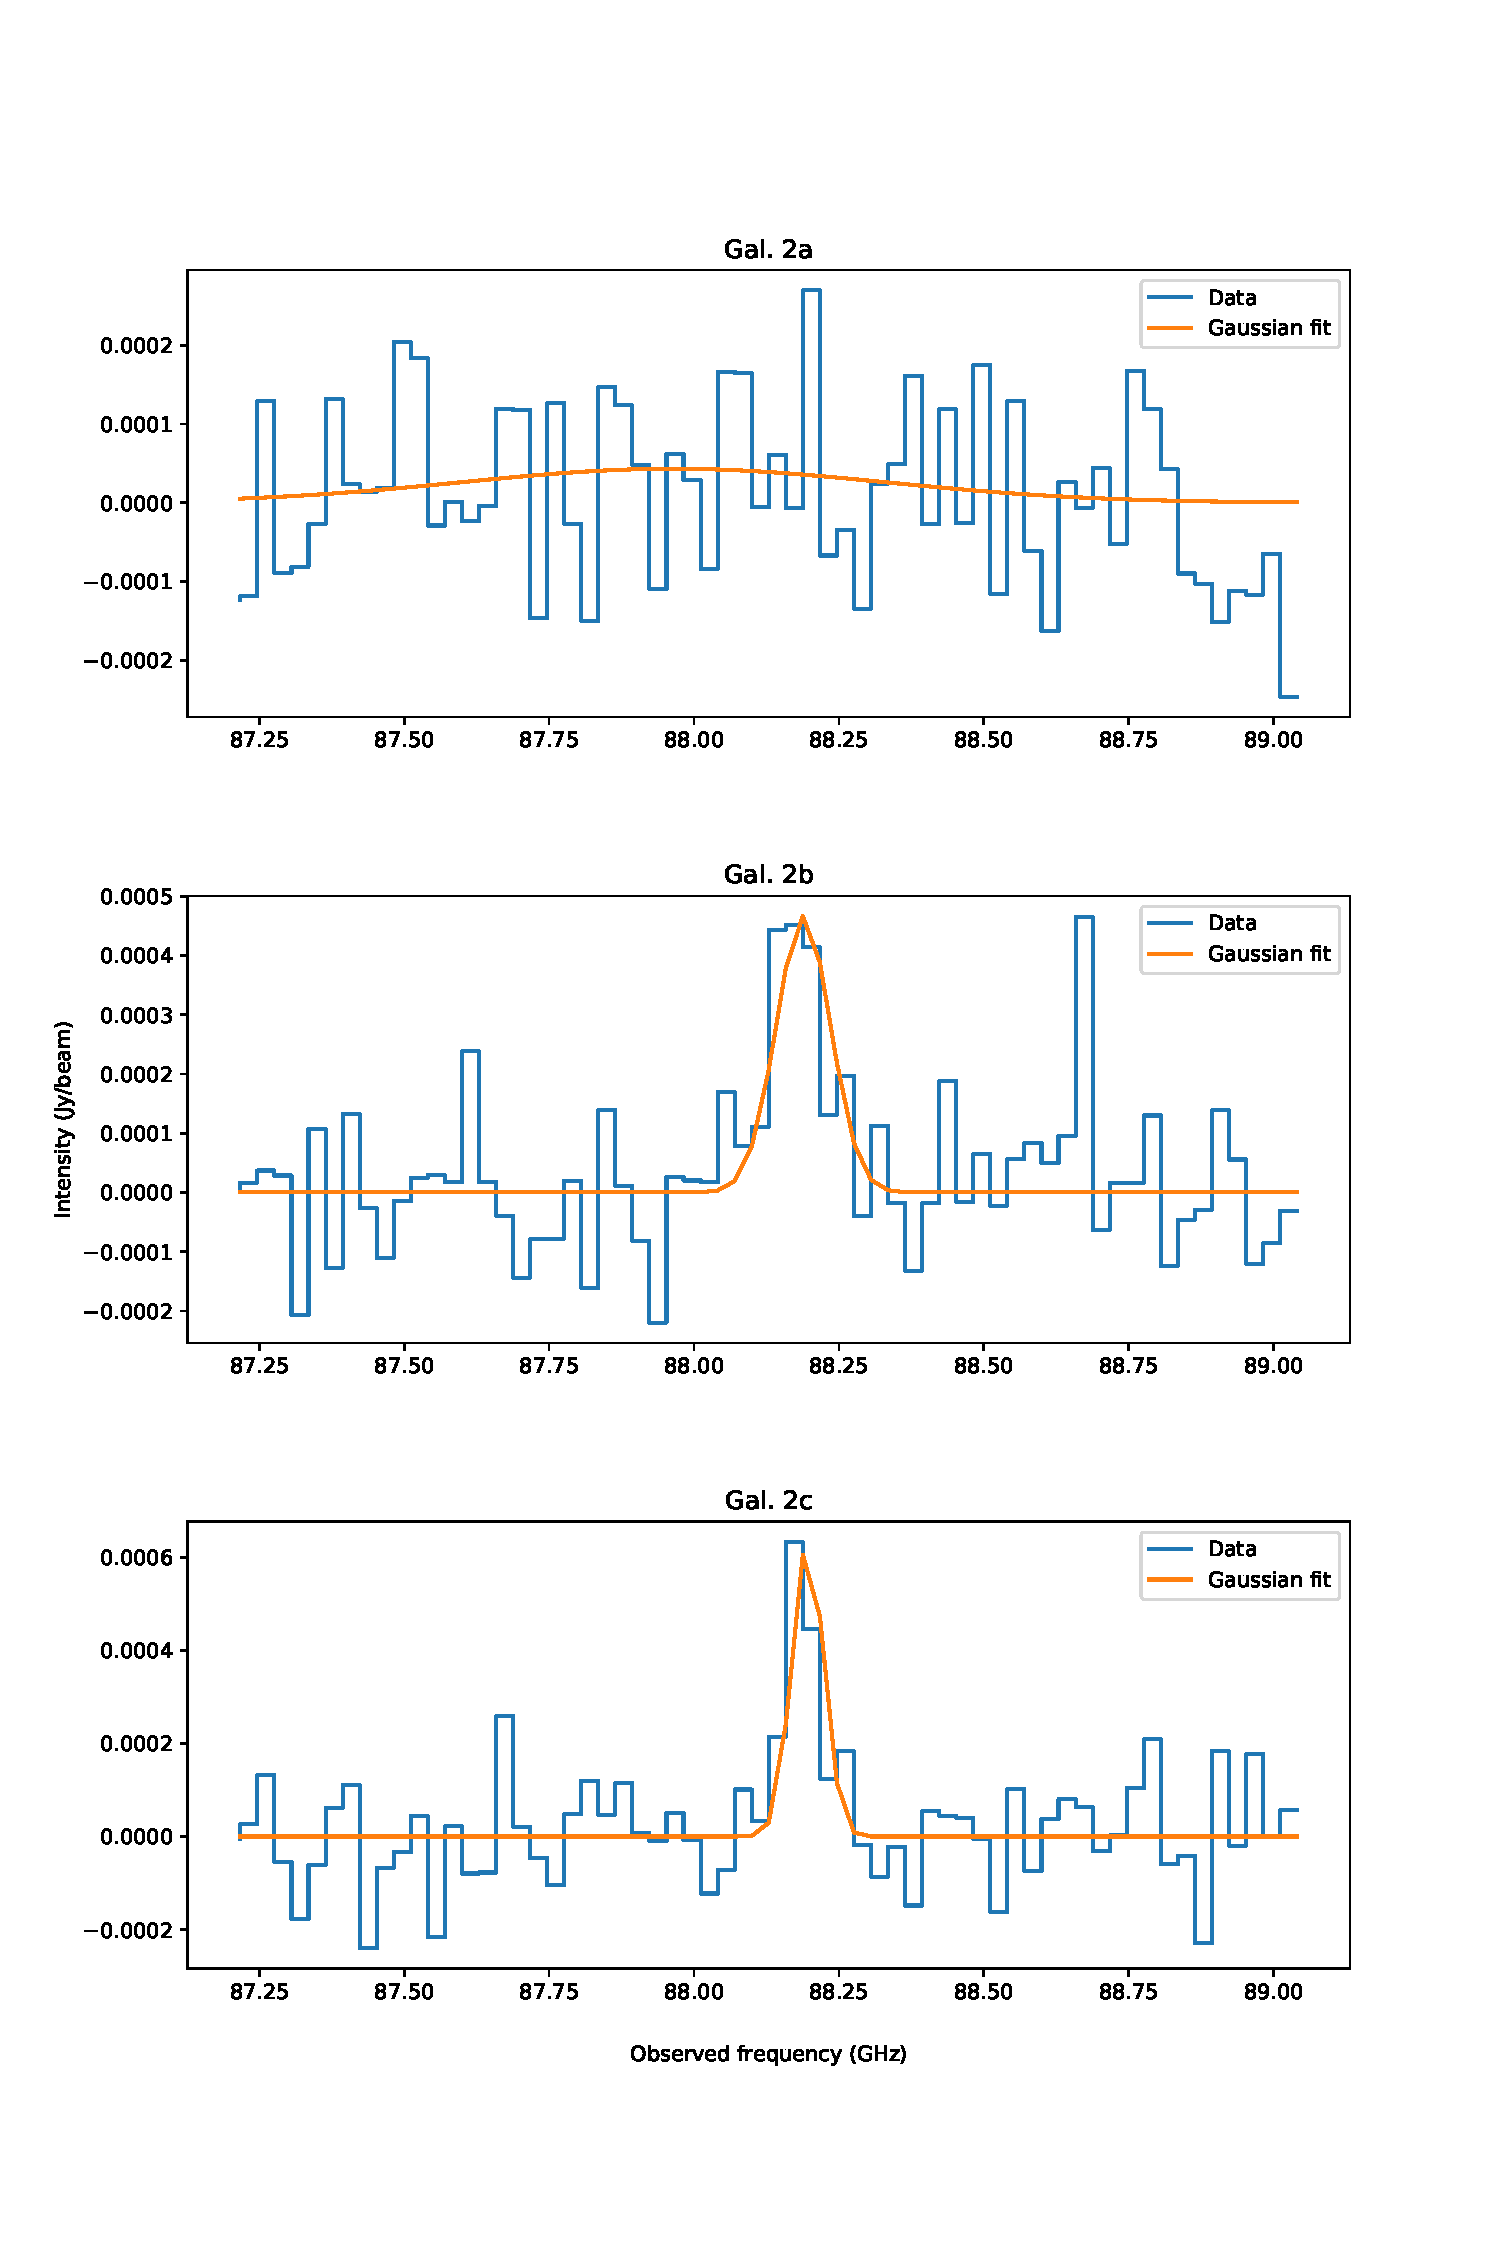
\includegraphics[width=0.8\linewidth]{../figs/gaussian_fit.pdf}
	\caption{Plot of the spectra of each lensed image, with a 1D Gaussian fit in orange.} 
    \label{fig:gaussian_fit}
\end{figure}

Spectroscopic redshift can be calculated for an object using the formula 
\begin{align}\label{eqn:redshift}
	z = \frac{v}{v_0} - 1,
\end{align}
where $v$ is the observed frequency and $v_0$ is the rest-frame frequency. In thie case, the target transition in these spectra is the $^{12}$CO(J=3-2) transition, which has a rest-frame frequency of 345.8 GHz \citep{Carilli2013}. The observed frequency for each of the images was taken to be the mean of the Gaussian fit. The results are given in Table \ref{table:peaks_zs}. They are in line with what is expected, accounting for uncertainties---Table 1 in \cite{MacKenzie2014} gives the redshift of Gal. 2 as $2.91\pm0.04$. 
}

Using the calculated spectroscopic redshift, it is possible to convert the observed frequencies into radio velocities. First, the rest frequency of the $^{12}$CO(J=3-2) transition is shifted so velocities are relative to a redshift (ie. the source has zero velocity):
\begin{align}\label{eqn:restfreq_shift}
	v_s = \frac{v_0}{z+1},
\end{align}
where $v_s$ is the shifted rest frequency, $v_0$ is the unshifted rest frequency, and $z$ is the redshift of the source. Then, the radio velocity is given by 
\begin{align}\label{eqn:radio_vel}
	V_{rad} = (1 - \frac{v}{v_s})c,
\end{align}
where $V_{rad}$ is the radio velocity, $v$ and $v_s$ are defined as before, and $c$ is the speed of light. Using the radio velocity, Fig. \ref{fig:velocity_axis} was created. Apart from the x-axis now being labelled with both radio velocity (bottom) and observed frequency (top), it is identical to Fig. \ref{fig:gaussian_fit}.

\begin{figure}[!htbp]
    \centering
    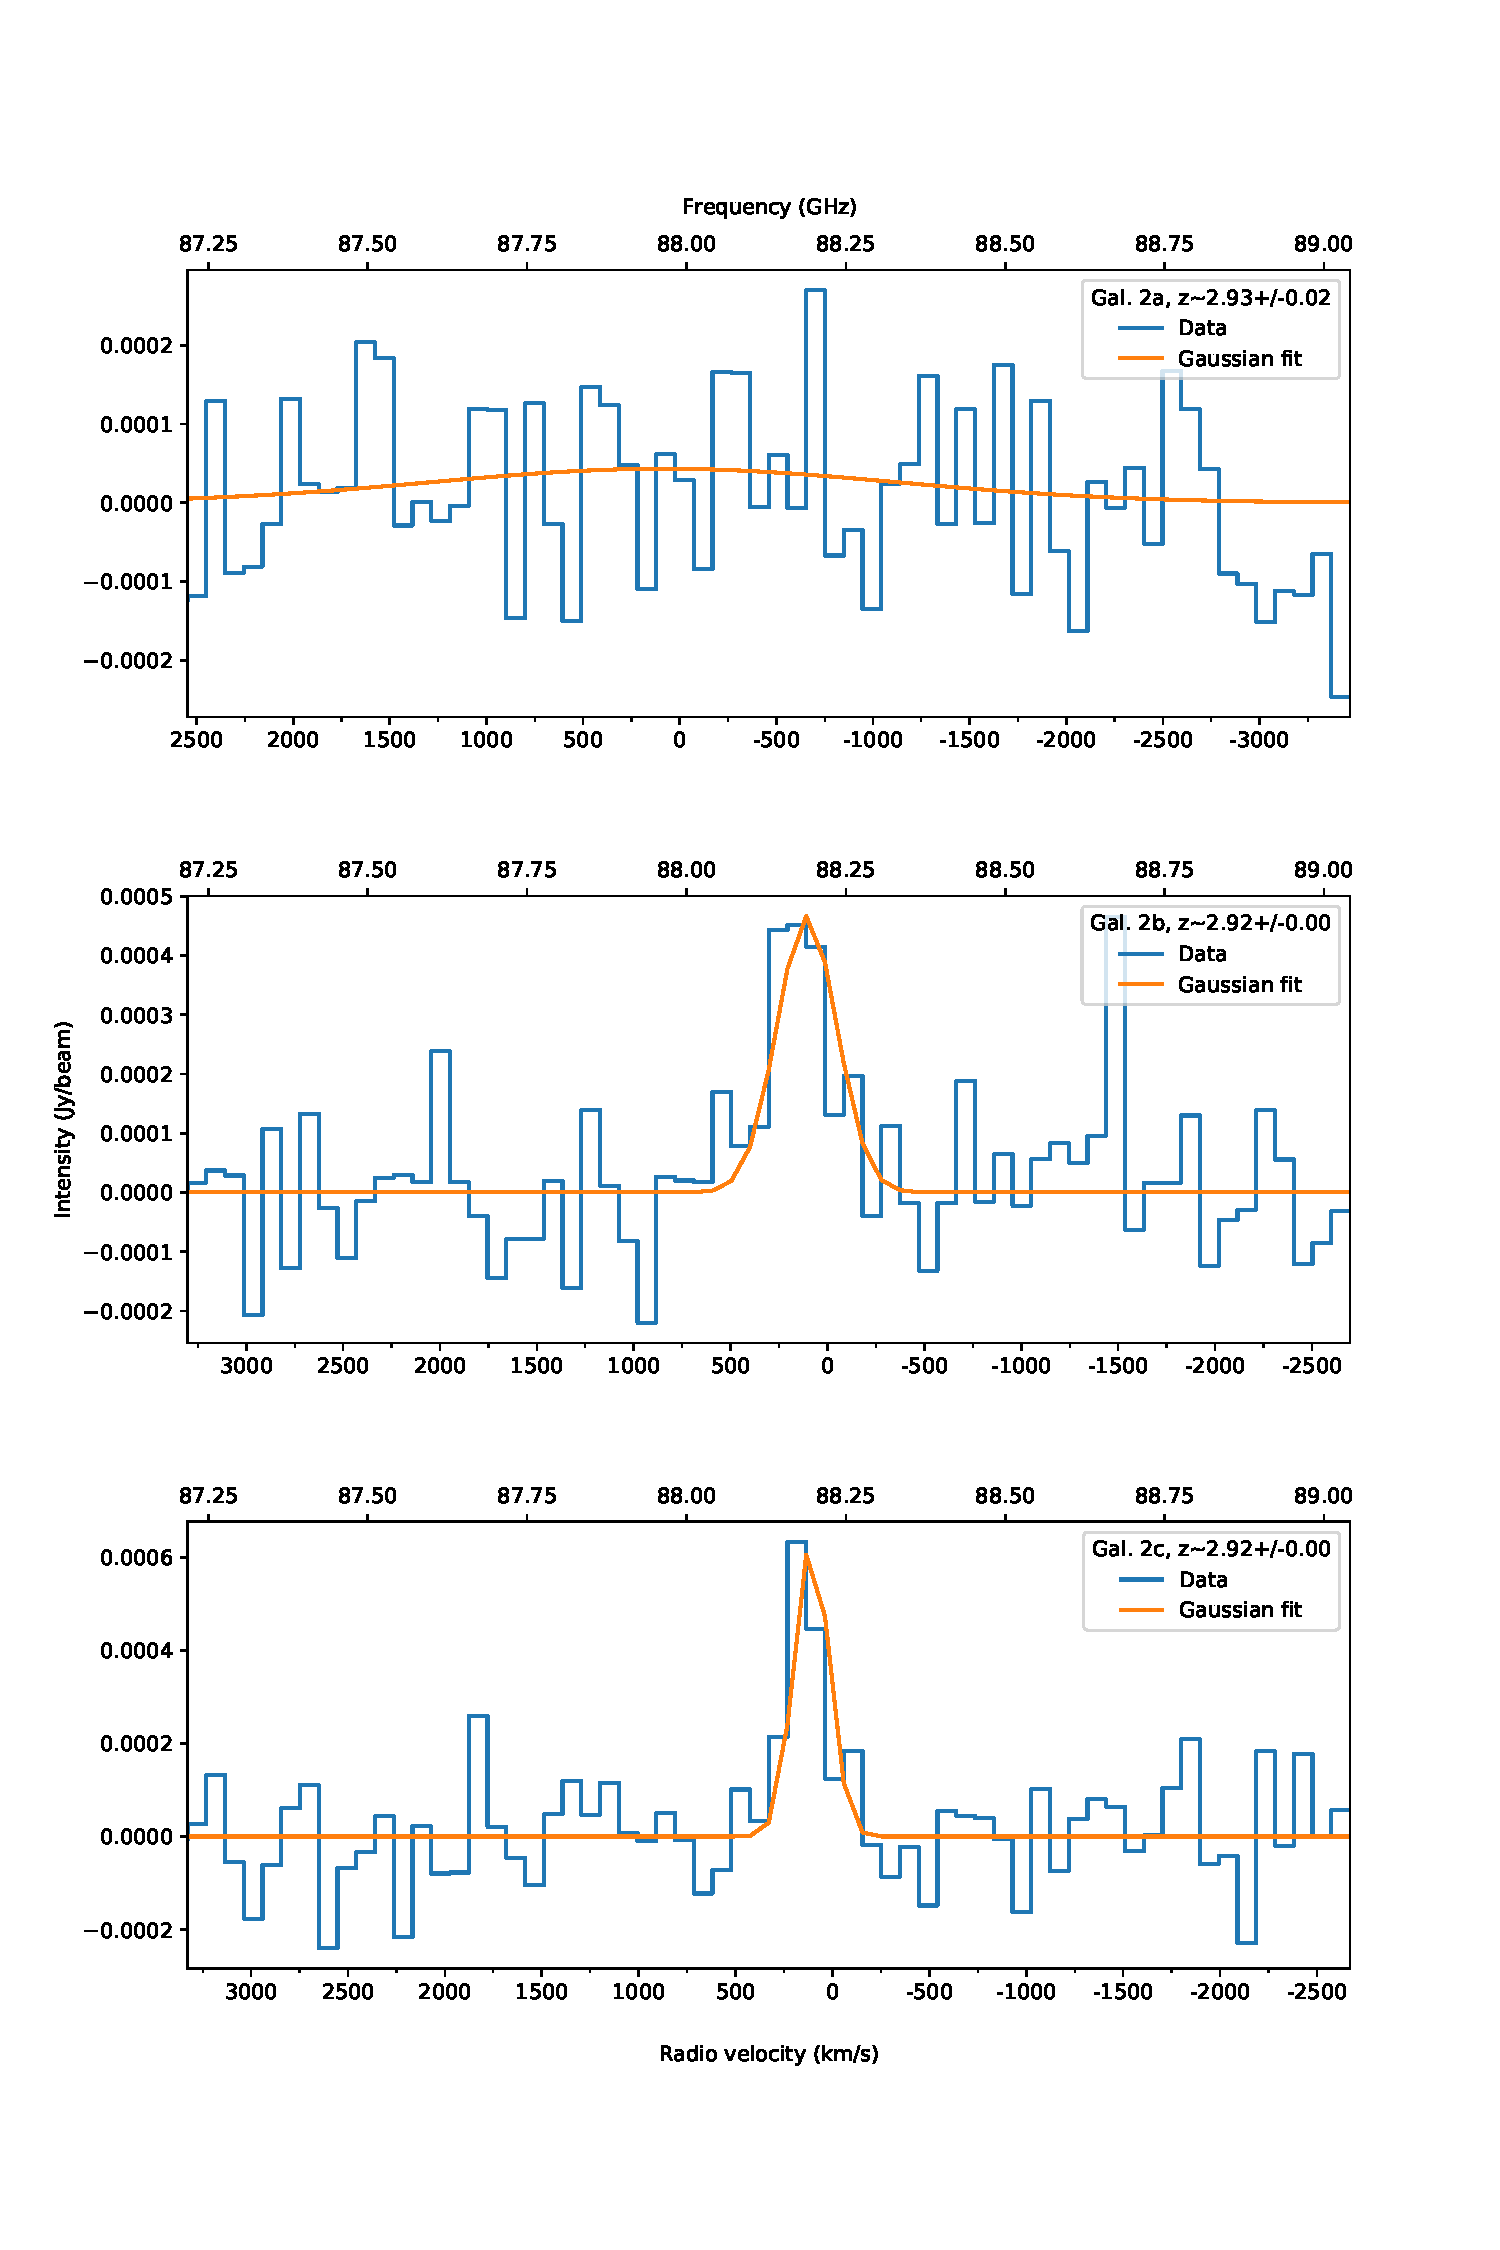
\includegraphics[width=0.8\linewidth]{../figs/velocity_axis_plot.pdf}
	\caption{Plot of the spectra with a 1D Gaussian fit (same as Fig \ref{fig:gaussian_fit}). Bottom x-axis is in radio velocity (km/s) with reference to the redshift to each image. Top x-axis is in observed frequency (GHz). y-axis is in intensity (Jy/beam). Note that the radio velocity increases going to the left, whereas the frequency increases going to the right.}
	\label{fig:velocity_axis}
\end{figure}

For each of the galaxies, the root mean square (RMS) of the intensity of the spectrum was calculated. This was done in order to better understand whether any line detections are merely noise or not. For the spectra of Gal. 2b and 2c, the line detections were masked out, and the calculation was done on the rest of the data. The equation for RMS, given $n$ data points $x_1, \ldots, x_n$, is 
\begin{align}\label{eqn:rms}
	\rm{RMS} = \sqrt{\frac{1}{n}\sum_i^nx_i^2}.
\end{align}

For each of the multiple images, the spectrum was perturbed with Gaussian noise in order to quantify the uncertainty in the measurements. In place of the measured intensity, a data point was sampled from a Gaussian distribution centered at the measured intensity with a standard deviation of the RMS error that was previously calculated. This yields a simulated spectrum, which was then fit according to the same procedure as for the original spectrum. These simulations were run 500 times for each image, which yielded a distribution of fit parameters. The mean of the 500 peak observed frequencies found by the fits are given in Table \ref{table:peaks_zs}. Since the assumption was made that the noise was Gaussian, the error on this parameter was taken to be the standard deviation of the peak observed frequencies. This process was repeated for the line width and the line flux (given in Table \ref{table:line_lum}).

\begin{figure}[!htbp]
    \centering
    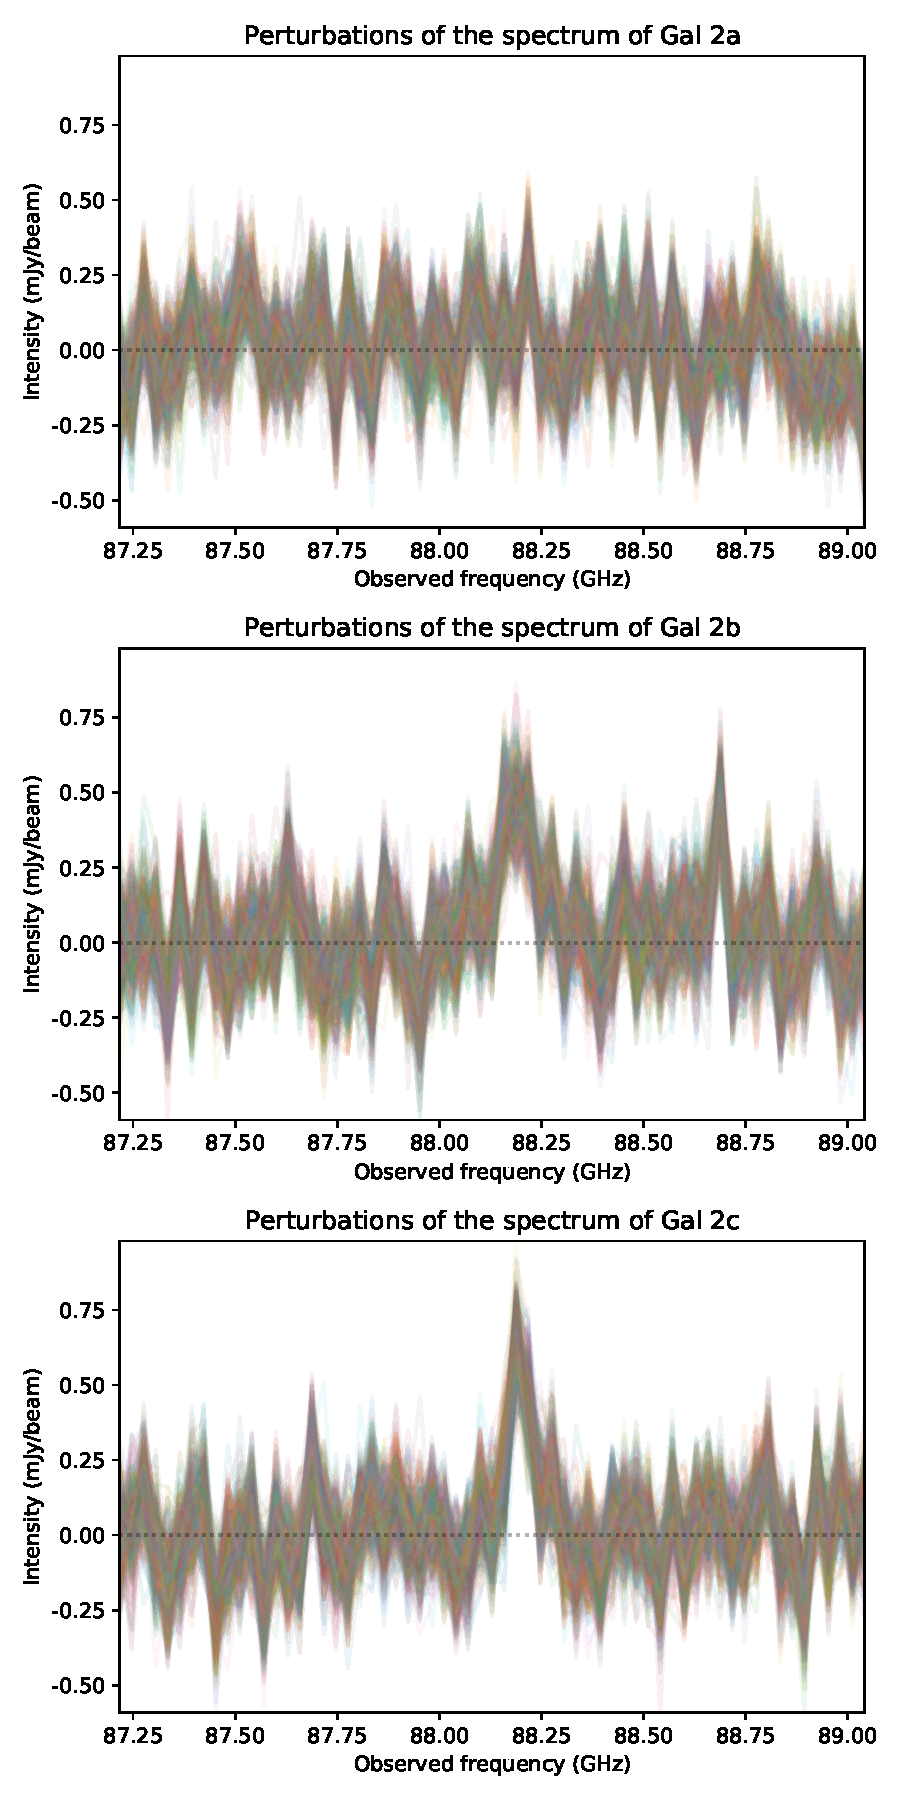
\includegraphics[width=0.6\linewidth]{../figs/perturbations.pdf}
	\caption{Plot of 500 realizations of the perturbed spectrum of each multiple image. The distribution of the errors was assumed to be Gaussian with a mean of the measured intensity and a standard deviation of the RMS error.}
	\label{fig:perturbations}
\end{figure}


\begin{table}[!htbp]
\begin{minipage}{\textwidth}
\centering
\begin{tabular}{ccccc}
\hline \\[-0.25cm]
Gal & Peak Observed Frequency & Line Width (FWHM) & RMSE & Redshift \\
ID  & GHz                     & ${\rm km\,s^{-1}}$      &      & \\[0.1cm]
\hline \\[-0.25cm]
2a & $88.14 \pm 0.17$\footnote{I know the significant digits are wrong for my uncertainties but I wanted a little more precision (otherwise everything ends up being a single digit later on when the errors propagate).} & $1956 \pm 1314$ & 1.11E-04 & $2.924 \pm 0.008$  \\
2b & $88.22 \pm 0.08$ & $768 \pm 880$  & 1.15E-04 & $2.920 \pm 0.003$\\
2c & $88.20 \pm 0.06$ & $502 \pm 1367$ & 1.08E-04 & $2.921 \pm 0.002$\\
\hline
\end{tabular}
\caption{Mean of the Gaussian fit, FWHM line width, RMS error, and redshift for each of the lensed images of Gal. 2.}
\label{table:peaks_zs}
\end{minipage}
\end{table}

\section*{Measuring Line Luminosity}

To obtain the line flux $S_{CO(3-2)}\Delta v$, the areas under the Gaussian curves for each of the spectra were integrated using Simpson's rule with the function \code{scipy.integrate.simps}. For the image without a clear emission detection, the flux was still calculated by integrating under the Gaussian profile, as \cite{Combes2007} finds this to yield results consistent within uncertainties. This was taken to be the upper limit of the line flux. 

Using the \code{astropy.cosmology} package, the luminosity distances $D_L$ to each of the images was calculated. The assumptions made were:
\begin{itemize}
	\item a flat $\Lambda$-CDM cosmology,
	\item Hubble's constant at $z=0$ of $H_0 = 70~\rm{km\,s^{-1}\,Mpc^{-1}}$,
	\item temperature of the cosmic microwave background (CMB) at $z=0$ of $T_{0_{CMB}} = 2.725~{\rm K}$, and
	\item density of non-relativistic matter at $z=0$, in units of the critical density, of $\Omega_M = 0.3$.
\end{itemize}

From the line flux and the luminosity distance, Eqn. 3 from \cite{Solomon1992} can be used to find the line luminosity:
\begin{align}\label{eqn:linelum}
	L'_{CO} = \frac{c^2}{2k}S_{CO}\Delta v \frac{D_L^2}{v^2 (1+z)^3},
\end{align}
where $L'_{CO}$ is the line luminosity and $k = 1.381\times 10^{-23}~{\rm J\,K^{-1}}$ is the Boltzmann constant. The line luminosity was computed for each of the images, and can be found in Table \ref{table:line_lum}.

\begin{table}[!htbp]
\centering
\begin{tabular}{cccc}
\hline \\[-0.25cm]
Gal & $S_{CO(3-2)}\Delta v$ & $D_L$ & $L'_{CO(3-2)}$ \\
ID  & $\rm{Jy\,km\,s^{-1}}$ & Mpc   & $\rm{K\,km\,s^{-1}\,pc^2}$ \\[0.1cm]
\hline \\[-0.25cm]
2a & $<(0.125 \pm 0.081)$ & $(2.464 \pm 0.003)\times 10^{4}$ & $<(5.25 \pm 3.42)\times 10^{9}$ \\
2b & $0.218 \pm 0.063$ & $(2.460 \pm 0.001)\times 10^{4}$ & $(9.15 \pm 2.64)\times 10^{9}$  \\
2c & $0.166 \pm 0.047$ & $(2.461 \pm 0.001)\times 10^{4}$ & $(6.96 \pm 1.99)\times 10^{9}$  \\
\hline
\end{tabular}
\caption{Line flux for the J=3-2 transition for $^{12}$CO, luminosity distance, and total line luminosity for each of the images.}
\label{table:line_lum}
\end{table}

\section*{Measuring Gas Mass}

For each of the images with a detectable emission line, the line luminosity of the $^{12}$CO(J=3-2) transition was used to estimate the line luminosity for the ground state transition $^{12}$CO(J=1-0). Table 2 in \cite{Carilli2013} gives the ratio $L'_{CO(3-2)} / L'_{CO(1-0)} = 0.27$ for the Milky Way. Under the assumption that the spectral energy distribution of the galaxy in question is similar to that the Milky Way, a simple rearrangement allows us to calculate the expected line luminosity for the ground state transition:
\begin{align}\label{eqn:ground_linelum}
	L'_{CO(1-0)} = \frac{L'_{CO(3-2)}}{0.27}.
\end{align}

We can use the conversion factor $\alpha_{CO}$, which gives the ratio of total molecular gas mass in $M_\odot$ to the total CO line luminosity in ${\rm K\,km\,s^{-1}\,pc^2}$, to calculate the apparent cold gas mass. Assuming a ratio similar to that of the Milky Way, the apparent cold gas mass is given by 
\begin{align}\label{eqn:gas_mass}
	M_{gas} = L'_{CO(1-0)} \alpha_{CO},
\end{align}
where $\alpha_{CO} = 4.6~{\rm M_\odot\,(K\,km\,s^{-1}\,pc^2)^-1}$ for the Milky Way. The gas mass is calculated using the line luminosities calculated for Gal. 2b and 2c and are given in Table \ref{table:gas_mass}.

In order to take into account the effects of gravitational lensing, the amplification factor for each image (from \cite{MacKenzie2014}, also given in Table \ref{table:gas_mass}) due to the lensing is used to calculate the delensed molecular gas mass of each image. Although the amplification factor is with respect to the flux density, all the calculations necessary to go from flux density to the gas mass are linear in the relevant variables (Eqn. \ref{eqn:linelum}, Eqn. \ref{eqn:ground_linelum}, Eqn. \ref{eqn:gas_mass}). Thus, we can directly apply the amplification factor to calculate the delensed gas mass. 

\begin{table}[!htbp]
\centering
\begin{tabular}{ccccc}
\hline \\[-0.25cm]
Gal & $L'_{CO(1-0)}$             & Apparent $M_{gas}$ & Amplification & Delensed $M_{gas}$ \\
ID  & $\rm{K\,km\,s^{-1}\,pc^2}$ & $M_\odot$          &               & $M_\odot$          \\[0.1cm]
\hline \\[-0.25cm]
2a & $<(1.94 \pm 1.27)\times 10^{10}$ & $<(8.94 \pm 5.83)\times 10^{10}$ & $2.86 \pm 0.04$ & $<(3.13 \pm 2.04)\times 10^{10}$ \\
2b & $(3.39 \pm 0.98)\times 10^{10}$  & $(1.56 \pm 0.45)\times 10^{11}$  & $8.1 \pm 0.4$   & $(1.92 \pm 0.56)\times 10^{10}$  \\
2c & $(2.58 \pm 0.74)\times 10^{10}$  & $(1.19 \pm 0.34)\times 10^{11}$  & $6.1 \pm 0.1$   & $(1.95 \pm 0.56)\times 10^{10}$  \\
\hline
\end{tabular}
\caption{Line luminosity for the ground-state J-transition of $^{12}$CO, apparent gas mass, and intrinsic (delensed) gas mass.}
\label{table:gas_mass}
\end{table}

To check whether the intrinsic gas masses calculated are consistent with each other across the multiple images, we take the difference between the computed values for Gal. 2b and 2c and normalize it by their average. Doing so, we find that the values are consistent to within 2\%: 
\begin{align}
	\frac{|M_{2b} - M_{2c}|}{\frac{M_{2b}+M_{2c}}{2}} = \frac{2.04\times 10^{8}}{1.94 \times 10^{10}} \simeq 1\%
\end{align}
where $M_{2b}$ and $M_{2c}$ are the intrinsic molecular gas masses calculated for Gal. 2b and 2c, respectively. 

\section*{Wrapping Up}

The simulations from Fig. \ref{fig:perturbations} are based on the assumption that errors are distributed normally. These simulations were used to generate the parameters seen in Table \ref{table:peaks_zs}, which then served as the basis for further calculations. These simulations were also used to quantify the uncertainty in the measurements, and it is possible that they were under or overestimated if the assumption does not hold. 

The conversion factor $\alpha_{CO}$, even within the Milky Way, only holds to a factor of two \citep{Carilli2013}. It is also uncertain that the assumption that the CO to molecular gas mass ratio of the galaxy in question is similar to that of the Milky Way: there are many factors to consider. For example, the metallicity and pressure of the interstellar medium (ISM) play an important role in determining $\alpha_{CO}$. Furthermore, with a far-infrared luminosity of $L_{FIR} = (6.7 \pm 0.6)\times 10^{11}~{\rm L_\odot}$, this galaxy can be classified as a luminous infrared galaxy (LIRG), for which the Milky Way conversion factor is unsuitably high \citep{Carilli2013}. 

There is also uncertainty in the CO excitation ladder (ie. the relative strengths of the observed rotational transitions), and thus the conversion factor from the line luminosity of the excited state $L'_{CO(3-2)}$ to that of the ground-state transition $L'_{CO(1-0)}$. Commonly used models (eg. large velocity gradient (LVG), photon-dominated regions (PDR), X-ray dominated regions (XDR)) for determining the excitation ladder---in addition to their underlying assumptions and intrinsic limitations---do not take into account that mid- and high-J CO emissions are enhanced by mechanisms other than collisions (eg. infrared pumping, radiative trapping) \citep{Carilli2013}. 

\begin{figure}[!htbp]
    \hspace{-1cm}
    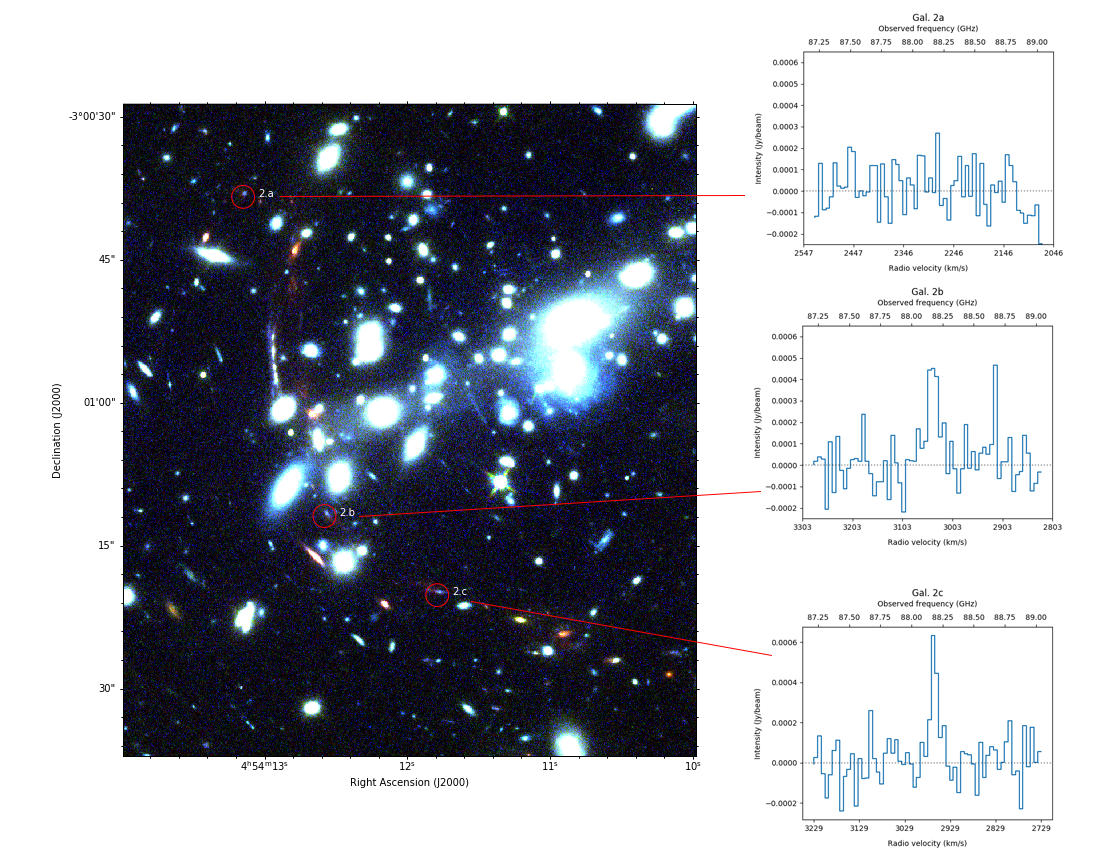
\includegraphics[width=1.1\linewidth]{../figs/final.png}
	\caption{RGB composite of MS 0451.6−0305 with F160W, F110W, and F814W filters, respectively. A percentile value of 99.85 was used to determine the maximum pixel value for the colourscale in the red and green channels, and a value of 99.0 was used in the blue channel. The multiple lensed images of Gal. 2 are indicated with white text. The spectra are extracted from circles with a diameter of 1", indicated in red. The bottom axes of the spectra are labelled in radio velocity, relative to the redshift calculated for each image, as given in Table \ref{table:peaks_zs}. The top axes are in observed frequency (GHz), and the side axes in intensity (Jy/beam).}
    \label{fig:final_oteo}
\end{figure}

The star formation rate (SFR) of this galaxy, as indicated in Table 2 of \cite{MacKenzie2014}, is ${\rm SFR}=99\pm9~{\rm M_\odot\,yr^{-1}}$. We can use this to calculate the star formation efficiency (SFE) using the equation
\begin{align}
	{\rm SFE} = \frac{\rm SFR}{M_{gas}}.
\end{align}
Using the values for $M_{gas}$ from Table \ref{table:gas_mass}, the SFE for each of the images was computed. The values are given in Table \ref{table:sfe}.

\begin{table}[!htbp]
\centering
\begin{tabular}{cc}
\hline \\[-0.25cm]
Gal & SFE \\
ID  & $\rm{yr^{-1}}$ \\[0.1cm]
\hline \\[-0.25cm]
2a & $<(3.17 \pm 2.09)\times 10^{-9}$ \\
2b & $(5.14 \pm 1.56)\times 10^{-9}$  \\
2c & $(5.09 \pm 1.53)\times 10^{-9}$  \\
\hline
\end{tabular}
\caption{Star formation efficiency as calculated from the delensed gas mass of each image.}
\label{table:sfe}
\end{table}

\newpage
\nocite{*}
\bibliography{sources}

\end{document}

